\documentclass[preprint,12pt]{elsarticle}

\usepackage[T1]{fontenc}
\usepackage[utf8]{inputenc}
\usepackage{amsmath,amssymb,amsthm}
\usepackage{booktabs}
\usepackage{multirow}
\usepackage{graphicx}
\usepackage{microtype}  % char protrusion / font expansion — minimises overfull boxes
\usepackage{subcaption}
\usepackage{algorithm}
\usepackage{algpseudocode}
\usepackage{hyperref}
\usepackage{orcidlink}
\usepackage{url}
\usepackage{enumitem}
\usepackage{mathtools}
\usepackage{setspace}
\usepackage[section]{placeins}  % keep floats within their section (no drift into References)

% Algorithm 1 runs to ~70 lines, about two pages: as a float it can never be
% placed ("Float too large for page"). This environment keeps the caption,
% numbering and rules of `algorithm` but page-breaks like ordinary text.
\makeatletter
\newenvironment{breakablealgorithm}
  {\begin{center}%
     \refstepcounter{algorithm}%
     \hrule height.8pt depth0pt \kern2pt%
     \renewcommand{\caption}[2][\relax]{%
       {\raggedright\textbf{\ALG@name~\thealgorithm}\ ##2\par}%
       \ifx\relax##1\relax
         \addcontentsline{loa}{algorithm}{\protect\numberline{\thealgorithm}##2}%
       \else
         \addcontentsline{loa}{algorithm}{\protect\numberline{\thealgorithm}##1}%
       \fi
       \kern2pt\hrule\kern2pt%
     }%
  }{\kern2pt\hrule\relax\end{center}}
\makeatother

% Shrink an over-wide table down to the text width; leave fitting tables at their natural size.
\newcommand{\fittable}[1]{\resizebox{\ifdim\width>\linewidth \linewidth\else \width\fi}{!}{#1}}

% Default \@makefntext only indents the first line (for the mark); wrapped
% continuation lines fall back to the page margin, so multi-line footnotes
% (e.g. the "Email addresses:" block, or any footnote spanning >1 line) look
% misaligned. Add a matching \leftskip so wrapped lines hang-indent flush
% with the first line's text.
\makeatletter
\long\def\@makefntext#1{%
  \parindent 1em\noindent
  \hangindent 1.8em\hangafter 1
  \hb@xt@1.8em{\hss\@makefnmark}#1}
\makeatother

\journal{Computers \& Operations Research}

\newtheorem{proposition}{Proposition}

\begin{document}

\begin{frontmatter}

\title{An Adaptive Large Neighborhood Search with Lagrangian Certification for the Selective Routing Problem with Synchronization}

\author[aff1]{David Chouchena\orcidlink{0009-0005-9871-1330}}
\ead{davidch@mail.sapir.ac.il}

\author[aff1]{Yuval Ben-Abu\corref{cor1}\orcidlink{0000-0002-6983-5730}}
\cortext[cor1]{Corresponding author}
\ead{yuvalb@sapir.ac.il}

\address[aff1]{Sapir Academic Institute, D.N. Hof Ashkelon 7915600, Israel}

\begin{abstract}
We study the Selective Routing Problem with Synchronization (SRPS), a
profit-maximising variant of the Team Orienteering Problem in which each
selected job must be served simultaneously by a prescribed subset of processors
under a global time limit (Riera-Ledesma and Salazar-Gonz\'alez, 2021). The exact
branch-and-price-and-cut (BPC) method proves many instances through $n=60$, but
leaves residual gaps on the hardest class and no reported results on larger
instances.

To the best of our knowledge, we develop the first ALNS-based,
Lagrangian-certified heuristic for SRPS. It returns a feasible synchronised
routing solution and a theoretically valid, independently checkable upper
bound, yielding a per-instance certified optimality gap. A
synchronisation-aware insertion procedure evaluates up to $5^{|K_j|}$
cross-route placements per job, and a warm-started subgradient scheme refreshes
the bound in-loop. A separately invoked post-search refinement re-solves the
dual for the final incumbent; it can tighten the certificate but never changes
the incumbent.

On the standard 660-instance benchmark ($|K_j|\in\{2,3,4\}$), the method
proves optimality on 446 instances (67.6\%); the mean certified gap is
0.066\%, the maximum is 1.614\%, 96.8\% of instances are certified within
0.5\%, and all are within 2\%. It recovers the BPC-proved optimum on 241 of
245 instances (98.4\%) and supplies certified solutions for all 415 instances
that BPC leaves open or unreported: 112 with a residual BPC gap, 300 with no
reported BPC result, and three partially solved cases. Among these, 196 have no
published BKS. Median per-instance wall-clock time is 6.2 minutes
within the same one-hour cap.
\end{abstract}

\begin{keyword}
selective routing \sep synchronization \sep adaptive large neighborhood search \sep Lagrangian relaxation \sep certified heuristic \sep orienteering
\end{keyword}

\end{frontmatter}

\section{Introduction}

The Selective Routing Problem with Synchronization (SRPS) arises in telescope scheduling at the Gran Telescopio Canarias, where observations require coordinated use of multiple shared resources under a global time budget \cite{RieraLedesma2021SRPS}; the broader problem of scheduling observations on instruments and telescope arrays under resource and time constraints is an active application area for operational-research methods \cite{Ma2025RadioTelescope}. SRPS asks which jobs to select, and in what processor routes to embed them, so as to maximise collected profit while ensuring that every selected multi-processor job is jointly served and scheduled feasibly.

SRPS belongs to the profit-collecting routing family \cite{Feillet2005TSPProfits} rooted in the Orienteering Problem (OP) \cite{Golden1987OP} and the Team Orienteering Problem (TOP) \cite{Chao1996TOP}, but differs from standard TOP by requiring joint service across subsets of processors \cite{Vansteenwegen2011Orienteering,Gunawan2016OPSurvey}. This synchronisation requirement creates a coupling between routes that destroys the separability exploited by most classical orienteering heuristics and exact methods.

Riera-Ledesma and Salazar-Gonz\'alez \cite{RieraLedesma2021SRPS} introduced SRPS together with an exact branch-and-price-and-cut (BPC) algorithm and a benchmark suite of eight instance families. Their method proves optimality for many instances, but on the hardest class it leaves nonzero primal--dual gaps at $n=60$; BPC provides no reported incumbent for these larger instances \cite{RieraLedesma2021SRPS}. At the same time, no heuristic or primal--dual approximation method has been proposed specifically for SRPS. We call our approach a \emph{Lagrangian-certified heuristic}: it returns a feasible primal solution together with a valid Lagrangian upper bound, yielding an instance-specific certified gap. This does not imply complementary slackness or a worst-case approximation ratio; those would constitute a \emph{primal--dual approximation algorithm}, which this method is not.

To the best of our knowledge, this paper develops the first ALNS-based Lagrangian-certified heuristic for SRPS that provides independently verifiable per-instance optimality gaps. The primal component is an Adaptive Large Neighborhood Search whose main problem-specific ingredient is a synchronisation-aware insertion procedure: inserting a $|K_j|=4$ job requires evaluating up to $5^4=625$ cross-route position combinations, each checked by a longest-path feasibility oracle. The Lagrangian component yields hard per-instance upper bounds and is re-tightened in-loop, so the method returns both a feasible solution and a certificate.

The contributions are fivefold:
\begin{enumerate}[label=(\roman*)]
    \item a problem-specific ALNS for SRPS with synchronisation-feasible insertion and adaptive runtime allocation;
    \item a Lagrangian relaxation of the joint-service coupling constraints that provides valid upper bounds and certified optimality gaps;
    \item an in-loop warm-started re-bounding mechanism that couples the current incumbent to Polyak step calibration, and which drives the stopping rule as well as tightening certificates on hard instances;
    \item a post-search refinement stage that recomputes the dual bound for the returned solution once the search has terminated, exploiting the fact that subgradient effort competes with the primal search inside the budget but not after it, and which raises the share of instances proved optimal from $42.4\%$ to $67.6\%$ without altering a single incumbent; and
    \item a computational study on 660 benchmark instances from six nontrivial SRPS families $(K=2,3,4)$, including new certified solutions for all open large instances and a statistical characterisation of instance hardness.
\end{enumerate}

Methodologically, the paper contributes to the line of work that couples heuristic
search with exact bounding schemes: we adopt a classical Lagrangian relaxation and
subgradient method to provide rigorous per-instance upper bounds, and embed this
dual mechanism tightly inside an SRPS-specific ALNS.

The method is intended not as a replacement for exact SRPS solvers but as a complement to them: it is designed to add value precisely on the instances an exact method leaves open --- those left with a residual gap at the time limit, or for which no result is reported --- while deferring to the exact solver wherever that solver terminates.

Families H1 and E1 $(|K_j|=1)$ reduce to TOP and are solved to optimality by BPC with negligible gaps \cite{RieraLedesma2021SRPS}; they are therefore excluded from the primary study so that the analysis focuses on the synchronisation-driven difficulty that motivates SRPS. Throughout the paper, a certified gap of $x$\% means that the returned solution is guaranteed to lie within $x$\% of optimal; it is an upper bound on suboptimality, not a direct distance-to-optimum measurement.

The remainder of the paper is organised as follows. Section~\ref{sec:problem} defines SRPS, gives a self-contained optimisation model, and positions the problem relative to related routing variants. Section~\ref{sec:related} reviews existing SRPS work and the benchmark taxonomy. Sections~\ref{sec:lagrangian} and \ref{sec:alns} present the Lagrangian bounding scheme and the adaptive ALNS, respectively. Section~\ref{sec:experiments} reports the computational results, and Section~\ref{sec:discussion} discusses their implications and scope. Section~\ref{sec:conclusion} concludes.

\section{Problem description}\label{sec:problem}

\subsection{Formal SRPS definition and notation}

Let $J=\{1,\dots,n\}$ denote the job set and $K$ the set of processors. Each job $j\in J$ yields profit $b_j$ and requires a subset $K_j\subseteq K$ of processors; symmetrically, $J_k=\{j\in J:k\in K_j\}$ denotes the jobs requiring processor $k$. Travel and processing times are given by a matrix $(t_{ij})$, where $i,j$ are route nodes (jobs or depots), and the planning horizon is bounded by a global time limit $L$.

SRPS seeks a set of elementary processor routes $P_k$ and a selected job set such that each selected job $j$ is served by every processor in $K_j$, all required processors start service at a common feasible time, and the global time limit is respected. The objective is to maximise the total collected profit $\sum_{j\in J} b_j y_j$.

\subsection{Binding constraints}

Before stating the model algebraically we name the three constraints it encodes,
because their interaction---particularly the second---is easy to misread.

\begin{enumerate}
  \item \textbf{Horizon.} Elapsed time from the start depot to the end depot may
    not exceed $L$ on any processor.
  \item \textbf{Synchronisation.} All processors in $K_j$ must start job $j$ at
    the same instant $s_j$. For every arc $(i\to \ell)$ traversed by any
    processor, $s_\ell-s_i\ge t_{i\ell}$. Processors may idle before a
    synchronised start, and \emph{that idle time counts toward $L$}.
  \item \textbf{Consistency.} If any processor serves $j$, every processor in
    $K_j$ must serve $j$. Partial service is forbidden.
\end{enumerate}

Constraints~2 and~3 are distinct requirements and are often conflated: consistency
says \emph{which} processors must serve a job, synchronisation says \emph{when}
they must do so. A solution can satisfy either without the other.

Constraint~2 is a difference-constraint system: earliest start times are given by
longest paths in the arc-weighted graph induced by the routes, and a cyclic graph
means no feasible schedule exists. This is what makes feasibility checkable in
linear time, and it is the check the heuristic of Section~\ref{sec:alns} uses. The
idle-time clause is what separates ``route length $\le L$'' from ``makespan $\le
L$'': routes that each fit comfortably inside the horizon may still be jointly
infeasible once synchronised waiting is charged.

\subsection{Optimisation model}

We adopt the compact arc-flow formulation SRPS-1 of Riera-Ledesma and
Salazar-Gonz\'alez \cite{RieraLedesma2021SRPS}. Its structure is what the
relaxation of Section~\ref{sec:lagrangian} acts on: per-processor routing
variables, a job-selection variable $y_j$, synchronisation of start times
across each job's required processors, a global horizon, and the joint-service
coupling $y_j \le x_{j,k}$ that links the two. The full formulation is given in the Supplementary Material.

\subsection{Relation to OP, TOP, and synchronisation variants}

SRPS reduces to TOP when $|K_j|=1$ for every job, so it inherits the prize-collecting routing structure of OP/TOP \cite{Vansteenwegen2011Orienteering}. The distinguishing feature is synchronisation: a selected job may require several processors to serve it jointly, creating inter-route coupling in both selection and timing.

Beyond SRPS, a large literature studies heuristics and exact methods for related orienteering and synchronised routing problems, including TOP and its time-window variants, clustered/team orienteering, and vehicle routing with synchronisation constraints \cite{Drexl2012SurveySync,Afifi2016COPTW}. Representative approaches combine branch-and-price, tabu search, large neighbourhood search, and hybrid metaheuristics, but generally do not provide per-instance optimality certificates for the returned solutions. SRPS inherits the profit-maximising structure of these problems while adding a joint-service coupling that removes the route separability exploited by most existing heuristics.

Close relatives differ in important ways. In clustered orienteering with time windows, teams are typically homogeneous and individual members cover separate tasks inside a cluster rather than jointly serving the same job. In synchronised VRPs, the focus is usually cost minimisation with mandatory service \cite{Drexl2012SurveySync,Afifi2016COPTW}, whereas SRPS is selective and profit maximising. Closely related prize-collecting routing problems with synchronisation have appeared recently --- two-echelon prize-collecting routing with vehicle synchronisation \cite{TwoEchelonPCVRPSync} and aquaculture service-vessel routing \cite{AquacultureServiceVRP} --- but these route vehicle fleets under two-echelon or mandatory-task structure rather than the per-job processor-subset coupling of SRPS. These differences justify treating SRPS as a distinct problem class rather than a routine variant of TOP or synchronised VRP.

\section{Existing work and benchmark instances}\label{sec:related}

\subsection{Exact work on SRPS}

The application that motivates SRPS decomposes into two tasks: a continuous problem of configuring the instrument, and the combinatorial decision of which observations to select and in what order to serve them. A heuristic exists for the former \cite{SalazarGonzalez2021Masks}; the latter is SRPS, and it has been addressed exactly but never heuristically. This paper takes up that second task. The SRPS literature is currently anchored by the branch-and-price-and-cut algorithm of Riera-Ledesma and Salazar-Gonz\'alez \cite{RieraLedesma2021SRPS}, built on a compact arc-flow formulation denoted SRPS-1. Two variants are reported: BPC-SRPS-E, which enhances the pricing step, and BPC-SRPS-N, a node-based alternative. The method is run with a 1 CPU-hour limit, and reports a primal--dual gap of $100\times(\text{dual}-\text{primal})/\text{primal}$.

Its performance establishes both the strength of the exact baseline and the motivation for a complementary primal--dual heuristic. In the hardest class-4 families, all instances up to $n\le 55$ are solved to optimality, but at $n=60$ nonzero gaps remain, reaching 1.64\% on the Euclidean family at $\alpha=0.75$ \cite{RieraLedesma2021SRPS}. For larger class-4 instances $(n\ge 65)$, no benchmark solutions are published. These two regimes --- hard instances with residual exact gaps, and larger instances with no reported exact result --- define the main space in which a certified heuristic can add value.

\subsection{Broader routing and primal--dual context}

The broader routing literature offers two complementary precedents for the present work. First, ALNS and related destroy--repair metaheuristics have proved effective across TOP, clustered orienteering, and VRP variants with rich side constraints, because they can combine strong primal search with problem-specific insertion logic \cite{RopkePisinger2006ALNS,PisingerRopke2007LNS,Vansteenwegen2011Orienteering,StochasticALNSPrizeCollecting}; a substantial body of metaheuristics---tabu search, variable neighbourhood descent, and guided local search among them---has been developed specifically for the team orienteering problem \cite{Archetti2007MetaheuristicsTOP,Tang2005TabuTOP,Bouly2010MemeticTOP,Vansteenwegen2009GLSTOP}, and recent reviews catalogue and rank the destroy and repair operators used across these applications \cite{ALNSOperatorReview}. Second, Lagrangian relaxation and subgradient schemes are classical tools for routing problems in which a small set of complicating constraints can be dualised to obtain decomposable subproblems and instance-specific upper bounds \cite{Fisher1981Lagrangian,Guignard2003Lagrangean,Held1974Subgradient,KohlMadsen1997VRPTW,Kohl1999LagrangeVRPTW}; more recently, matheuristics that interleave such relaxations with metaheuristic search have become an established way to obtain both strong primal solutions and bounds for routing problems \cite{ArchettiSperanza2014Matheuristic}.

What is missing in the SRPS setting is the combination of these two traditions.
Existing SRPS work is exact and benchmark-defining, but does not provide a scalable
heuristic counterpart \cite{RieraLedesma2021SRPS}. Existing TOP and
synchronised-routing heuristics offer powerful primal search machinery
\cite{RopkePisinger2006ALNS,Vansteenwegen2011Orienteering,Drexl2012SurveySync,Afifi2016COPTW},
and Lagrangian relaxations are widely used to derive strong dual bounds in vehicle
routing \cite{KohlMadsen1997VRPTW,Kohl1999LagrangeVRPTW}, but to the best of our
knowledge there is no method that embeds an ALNS inside an in-loop Lagrangian
certification scheme providing per-instance optimality gaps for SRPS; we are not aware
of an analogous certified heuristic for closely related synchronised routing problems
either, though we make no claim to an exhaustive survey of that broader literature.
The present method is designed to supply exactly
that combination, embedding a Lagrangian upper bound directly inside an
SRPS-specific ALNS.

\subsection{Benchmark instance families}

Table~\ref{tab:families} summarises the benchmark taxonomy introduced in \cite{RieraLedesma2021SRPS}. The full benchmark contains 960 instances. The primary study covers the six nontrivial families H2--H4 and E2--E4, i.e. 660 instances, where synchronisation is essential because $|K_j|\ge 2$. Families H1 and E1 are omitted from the main analysis because they reduce to TOP and would dilute the synchronisation-driven signal; they are retained only as a supplementary large-scale check.

\begin{table}[t]
\centering
\caption{SRPS benchmark families.}
\label{tab:families}
\resizebox{\textwidth}{!}{%
\begin{tabular}{lcccccccc}
\toprule
Label & Prefix & Class & $|K_j|$ & Distance & $n$ range & Groups & $\alpha$ values & Coverage \\
\midrule
H1 & A  & 1 & 1 & Line      & 400--500 & 25 & 3 & full \\
H2 & B  & 2 & 2 & Line      & 100--150 & 30 & 3 & full \\
H3 & C  & 3 & 3 & Line      & 50--80   & 35 & 3 & full \\
H4 & D  & 4 & 4 & Line      & 40--80   & 45 & 3 & up to $n\le 60$ \\
E1 & EA & 1 & 1 & Euclidean & 150--500 & 75 & 3 & full \\
E2 & EB & 2 & 2 & Euclidean & 100--150 & 30 & 3 & full \\
E3 & EC & 3 & 3 & Euclidean & 50--80   & 35 & 3 & full \\
E4 & ED & 4 & 4 & Euclidean & 40--80   & 45 & 3 & partial beyond $n=60$ \\
\bottomrule
\end{tabular}%
}
\end{table}

\noindent The parameter $\alpha\in\{0.25, 0.50, 0.75\}$ is the \emph{budget tightness ratio}: the global time horizon is $L = \alpha \cdot T$, where $T$ is a reference travel time derived from the instance geometry following \cite{RieraLedesma2021SRPS}. Smaller $\alpha$ imposes a tighter time budget (harder instances); larger $\alpha$ is more permissive. Line families use Euclidean-grid distances; Euclidean families use random-point distances. The distinction matters because Euclidean instances have more variable travel times, which amplifies the synchronised-idle-time difficulty.

\section{Lagrangian relaxation and dual bounding}\label{sec:lagrangian}

Lagrangian relaxation and subgradient optimisation are classical ingredients of primal--dual heuristics for routing problems: a complicating coupling is dualised, the problem decomposes into easier subproblems, and the resulting dual value provides an upper bound that can certify incumbent quality \cite{KohlMadsen1997VRPTW,Kohl1999LagrangeVRPTW}. The SRPS setting is especially suitable for this strategy because the joint-service coupling binds otherwise independent processor routes. The present method uses the resulting Lagrangian bound not as a one-off pre-processing device, but as a live in-loop certificate that guides termination.

\subsection{Relaxation formulation}

The complicating constraints are the joint-service couplings
\[
y_j \le x_{j,k} \qquad \forall j\in J,\; k\in K_j,
\]
which require that a job earns profit only if every required processor serves it. Relaxing these constraints with multipliers $\mu_{j,k}\ge 0$ yields the Lagrangian function
\[
L(\mu) = \sum_{j\in J} \max\Bigl(0, b_j - \sum_{k\in K_j}\mu_{j,k}\Bigr) + \sum_{k\in K} O_k(\mu),
\]
where $O_k(\mu)$ is the optimum of a single-processor orienteering problem in which job $j\in J_k$ carries the modified profit $\mu_{j,k}$; the Supplementary Material gives the expanded derivation of this decomposition and the exact dynamic-programming recurrence. Each $O_k(\mu)$ is solved \emph{exactly}---with no pruning, sampling, or candidate-set restriction---by bitmask dynamic programming in $O(2^{|J_k|}\,|J_k|^2)$. The exponential factor is bounded by a small constant rather than by $n$: because every job requires only $|K_j|\in\{2,3,4\}$ of the $|K|=55$ processors, the jobs spread thinly and each processor serves only a handful. The resulting bound on $|J_k|$ is small and does not grow with $n$; the measured distribution, and the cost it implies, are reported in Section~\ref{sec:experiments}.

Two properties of $O_k(\mu)$ matter for interpreting the certificates that follow.
First, each subproblem is solved to optimality, so no looseness in the bound
originates there, and validity does not depend on how far the subgradient has
converged: a short dual run yields a loose certificate, never an invalid one.
Second, the subproblem's time matrix charges the processing time of a job plus
the travel to the next, and enforces route length $\le L$; it is therefore
structurally blind to the synchronised idle time of constraint~2, because each
processor is solved in isolation. The relaxed solution is optimistic in that
specific, identifiable way, and it is the principal source of the residual
looseness reported in Section~\ref{sec:experiments}.

For every multiplier vector $\mu\ge 0$, the value $L(\mu)$ upper-bounds the optimal SRPS profit. The algorithm therefore minimises $L(\mu)$ over $\mu\ge 0$ by projected subgradient descent and records the best value encountered as the Lagrangian upper bound $UB_{\text{lag}}$.

To make the bound argument self-contained, we state the relaxed feasible set explicitly. Let $\mathcal{X}^{\mathrm{rel}}$ denote the set obtained from the SRPS feasible region by removing the joint-service coupling constraints while retaining all per-processor routing constraints (elementarity, time-horizon $L$, and depot return):
\begin{multline*}
\mathcal{X}^{\mathrm{rel}} = \bigl\{(y,x,\{P_k\}) \mid y\in\{0,1\}^n,\ P_k\text{ elementary and feasible within }L,\\
 x_{j,k}\text{ induced by }P_k\bigr\}.
\end{multline*}
Every SRPS-feasible solution belongs to $\mathcal{X}^{\mathrm{rel}}$, since removing constraints only enlarges the feasible set. The Lagrangian function is then the maximum over $\mathcal{X}^{\mathrm{rel}}$:
\[
L(\mu) = \max_{(y,x,\{P_k\})\in\mathcal{X}^{\mathrm{rel}}} \biggl[\sum_{j\in J} b_j y_j + \sum_{j\in J}\sum_{k\in K_j}\mu_{j,k}(x_{j,k}-y_j)\biggr],
\]
which decomposes by processor because the relaxed objective separates over the $P_k$.

\begin{proposition}[Validity of the Lagrangian bound]\label{prop:main_valid}
Let $z^*_{\mathrm{SRPS}}$ denote the optimal SRPS objective value, and let $L(\mu)$ be defined as above for any $\mu\ge 0$. Then:
\begin{enumerate}[label=(\alph*)]
  \item every SRPS-feasible solution belongs to $\mathcal{X}^{\mathrm{rel}}$;
  \item for every SRPS-feasible solution, $\sum_{j,k\in K_j}\mu_{j,k}(x_{j,k}-y_j)\ge 0$, so its objective does not exceed $L(\mu)$;
  \item therefore $z^*_{\mathrm{SRPS}} \le L(\mu)$ for every $\mu\ge 0$; and
  \item the maximisation over $\mathcal{X}^{\mathrm{rel}}$ decomposes into the job-selection terms and the per-processor orienteering subproblems $O_k(\mu)$ stated above.
\end{enumerate}
Consequently, $UB_{\mathrm{lag}} := \inf_{\mu\ge 0} L(\mu)$ is a valid upper bound on the optimum.
\end{proposition}

\begin{proof}
(a) Removing constraints only enlarges the feasible set. (b) Any SRPS-feasible solution has $y_j\le x_{j,k}$ for all $k\in K_j$, so each penalty term $\mu_{j,k}(x_{j,k}-y_j)\ge 0$. (c) Follows from (a) and (b) by maximising over SRPS-feasible solutions. (d) The multiplied objective decomposes as: the job-selection term $\sum_j (b_j-\sum_{k\in K_j}\mu_{j,k})y_j$ (optimal in closed form over $y$) and the per-processor terms $\sum_{k\in K}\mu_{j,k}x_{j,k}$ (each solved independently as a single-processor orienteering subproblem $O_k(\mu)$). Taking the infimum over $\mu\ge 0$ completes the argument.
\end{proof}

\subsection{Subgradient scheme}\label{sec:subgradient}

Multipliers are initialised by a fair profit split $\mu_{j,k}=b_j/|K_j|$, which makes the initial relaxed objective coincide with an independent-orienteering-style bound. The dual is then tightened by projected subgradient descent with Polyak-style step sizes \cite{PolyakStepSize},
\[
\eta_t = \frac{L(\mu_t)-\theta^*}{\|g_t\|^2},
\]
clamped for stability, with a diminishing fallback schedule when progress stalls. The lower reference value $\theta^*$ is the current incumbent $z^*$ throughout---initially the greedy solution, then the refreshed incumbent during in-loop re-bounding. The method uses no published best-known value.

The subgradient components are
\[
g_{j,k}=x^*_{j,k}-y^*_j,
\]
with projected updates $\mu_{j,k}\leftarrow \max(0,\mu_{j,k}-\eta_t g_{j,k})$. At each iteration the method solves all processor-specific subproblems, evaluates the subgradient, and updates the multipliers. The best bound found over the iteration budget is returned together with the corresponding multiplier vector, which is retained as a warm start for the next invocation.

\subsection{Certification logic}\label{sec:certification}

The algorithm proceeds in four stages on each instance:
\begin{enumerate}
    \item compute an initial upper bound from decomposed routing relaxations;
    \item run adaptive ALNS phases to improve the primal incumbent $z^*$;
    \item whenever the primal search stalls, invoke a warm-started Lagrangian re-bound using $\theta^*=z^*$; and
    \item track the certified gap
\end{enumerate}
\[
\text{cert\_gap} = \frac{UB_{\text{lag}}-z^*}{UB_{\text{lag}}}\times 100,
\qquad UB_{\text{lag}} = \bigl\lfloor \min_t L(\mu_t) + \varepsilon \bigr\rfloor,\quad \varepsilon=10^{-9},
\]
and stop when the upper bound matches the incumbent, the certified gap falls below 0.3\%, or the escalation tiers are exhausted.

The floor is applied before the gap is computed and is valid because all profits
$b_j$ are integral, so no feasible objective value lies strictly between
$\lfloor L(\mu)\rfloor$ and $L(\mu)$. It is not a cosmetic rounding: a dual
improvement smaller than one profit unit leaves the certified gap unchanged, so
the certificate advances in integer steps even when the underlying real-valued
bound improves continuously. In floating-point execution, the $\varepsilon=10^{-9}$
safeguard prevents a downward roundoff at an integer boundary; four instances
need it in the production float64 calculation, while the independent directed-
rounding re-derivation validates all 660 certificates with zero tolerance. The denominator $UB_{\text{lag}}$ is zero only if
the optimal SRPS profit itself is zero (no job can feasibly be served on that
instance); no instance in the benchmark studied here reaches this degenerate
case, and we do not encounter it, but note it for completeness since the gap
formula is otherwise undefined there.

The method is fully independent of any published benchmark value --- the
subgradient's reference value is the greedy construction before any search has
run, and the incumbent thereafter, so no external value enters at any point:
both the ALNS and
the Lagrangian dual reference use only the current incumbent, so no benchmark
solution enters the algorithm. Published BKS values are used solely for the
BEAT/TIE/GAP comparison in Section~\ref{sec:experiments}.

A certified gap of $x$\% means that the returned solution is guaranteed to lie within
$x$\% of the true optimum, because $UB_{\text{lag}}$ is a valid Lagrangian upper
bound and $z^*$ is a feasible SRPS objective value. A certified gap of $0$\% means
that the incumbent equals a valid Lagrangian upper bound; by weak duality
(Proposition~\ref{prop:main_valid}) this \emph{proves} the incumbent optimal, and we
accordingly call such instances \emph{proven optimal}. The number of instances certified
optimal in this sense, and their overlap with those the exact method closes, are
reported with the other computational results in Section~\ref{sec:experiments}.

\subsubsection*{Post-search certificate refinement}

disappears: once the search has terminated, additional subgradient iterations
draw only on budget the one-hour cap left unused by the primal stopping rule,
rather than on budget that would otherwise have gone to further primal search;
The bound and search are coupled only through the scalar reference $\theta^*$.
After search terminates, the refinement stage re-solves the Lagrangian dual for
the final incumbent using a larger iteration budget (3000 rather than 200
steps), skipping instances already certified exact, and reports
\[
UB^{\ast} = \min\bigl(UB_{\text{lag}},\ \bigl\lfloor L(\mu^{\ast}) + \varepsilon \bigr\rfloor\bigr),
\]
deterministic---the refined bound is a function of the instance, the iteration
the minimum of two valid upper bounds. Validity follows from
Proposition~\ref{prop:main_valid} for every $\mu\ge0$; the stage changes neither
the incumbent nor an objective comparison, only the certificate. Its runtime is
included in the per-instance one-hour accounting. The refinement effect and
iteration-cap sensitivity are reported in Section~\ref{sec:experiments} and the
Supplementary Material, respectively.

\subsection{In-loop warm re-bounding}

A single pre-search subgradient run can leave certificates loose on the hardest instances, especially at tight budgets and larger $n$. The adaptive loop therefore refreshes the dual bound \emph{inside} the search whenever a phase fails to improve the incumbent. Each re-bound is capped at 200 subgradient iterations or 60 seconds, is warm-started from the multiplier vector attaining the best bound so far (Section~\ref{sec:subgradient}), and uses the current incumbent as the Polyak target.

This coupling matters because once the primal search has already found a strong incumbent, the quantity $L(\mu)-z^*$ approximates the true residual optimality gap more closely than a cold lower reference does. Step sizes become more informative, the dual converges faster toward a useful certificate, and the updated bound directly governs whether further search is worthwhile. Empirically, this in-loop mechanism is particularly important on the hard tail of the benchmark, where a single pre-search bound leaves the loosest certificates; on those instances the refreshed bound is what closes the residual gap.

The archived 660-instance driver contains one historical implementation detail:
after a re-bound it assigns the newly computed valid bound rather than retaining
the minimum of the old and new bounds. On 10 instances this replaces the initial
decomposition bound by a looser valid bound, so it can only widen a reported gap
(by $0.0007$ percentage points in the 660-instance mean), never create a false
optimality claim. Algorithm~\ref{alg:solver} states the monotone rule used for
the post-search refinement. We retain the historical driver unchanged so the
archived campaign remains reproducible; future campaigns should retain
$\min(UB,UB')$ throughout.

\paragraph{Design choice: the coupling is narrow in both directions}
\label{sec:alns-lb-coupling}
The Lagrangian relaxation of Section~\ref{sec:lagrangian} is not a one-off
pre-processing device, but a dual mechanism tightened continuously around
the current incumbent: each ALNS phase attempts to improve $z^*$, and whenever a
phase fails to improve it, an in-loop Lagrangian re-bound is triggered,
warm-started from the multipliers that attained the best bound so far and using
the current incumbent as the Polyak reference $\theta^* = z^*$
(Section~\ref{sec:subgradient}). Stating where the coupling stops matters as
much as stating where it acts. The incumbent reaches the dual only through the
scalar level reference $\theta^*$: its selection structure is never communicated,
and multipliers are re-initialised from the previous dual solve rather than from
the primal solution. Symmetrically, the dual returns only a bound; the multipliers
themselves never enter operator selection, insertion scoring, or the destroy
criterion. Both channels are deliberately absent in the configuration evaluated
here, and widening either is a design question rather than a tuning question.

\section{Adaptive Large Neighborhood Search}\label{sec:alns}

\subsection{Representation and feasibility}

A solution consists of a selected job set and one elementary route per processor. Feasibility is verified by a \emph{synchronisation feasibility oracle} based on a longest-path schedule check, which we describe formally because it is the component that handles the defining difficulty of SRPS.

\subsubsection*{Feasibility oracle}

Given a candidate solution $(\textit{selected}, \{P_k\})$, the oracle builds a directed constraint graph with \emph{one node per selected job} plus depot nodes $\textit{start}, \textit{end}$ --- not one node per processor visit. Every consecutive pair $(i,i')$ on any processor's route contributes an arc $i\to i'$ weighted by the transition time $T_{i,i'}$ (processing time of $i$ plus travel to $i'$); an identical arc recurring on a second processor is not duplicated. Because a multi-processor job $j\in K_j$, $|K_j|\ge2$, is a single shared node, it receives one incoming arc from its predecessor on \emph{each} required processor, and the longest-path relaxation below takes the maximum over all of a node's incoming arcs. This is the entire synchronisation mechanism: no separate cross-processor arc construction is needed beyond the shared node, since the max-relaxation already enforces that $j$'s earliest start is the latest arrival among the processors required to serve it, with the resulting idle time absorbed automatically by each route's own subsequent arc weights.

Feasibility is then a longest-path computation: a topological sort (Kahn's algorithm) both detects any directed cycle --- which would mean some processor must serve a job before its own predecessor, an unconditional infeasibility --- and, if the graph is acyclic, orders a single relaxation pass that computes every node's earliest start time exactly in one sweep. The solution is feasible iff no cycle exists and the resulting earliest completion time at $\textit{end}$ does not exceed the horizon $L$. With $|V|=O(|\textit{selected}|)$ and $|E|=O\bigl(\sum_j|K_j|\bigr)=O(|\textit{selected}|)$ since $|K_j|\in\{2,3,4\}$ is bounded, both steps run in $O(|\textit{selected}|)$ time. The full construction, the cycle-detection argument, a worked two-processor synchronisation example, and the pseudocode (Algorithm~S2, \textsc{LongestPathScheduleCheck}) are given in the Supplementary Material.

This oracle is structurally blind to the synchronisation idle time induced by constraint~2: each per-processor subproblem in the Lagrangian relaxation is solved in isolation and therefore cannot represent the shared start requirement. This asymmetry---exact feasibility checking in the primal, optimistic relaxation in the dual---is the principal source of residual certificate looseness, and it is identifiable: it lives in the Lagrangian subproblem, not in any approximation in the search itself.

\subsection{Destroy operators}

Three destroy operators are used: random destroy, worst destroy, and Shaw destroy. The random operator removes a uniformly sampled subset of selected jobs; worst destroy removes the $d$ currently selected jobs with lowest profit $b_j$ (equivalently, highest marginal cost $-b_j$); and Shaw destroy picks a uniform-random pivot job $p$ from the selected set and removes the $d$ selected jobs with smallest relatedness $\rho(p,j) = T_{p,j}+T_{j,p}$ (round-trip transition time), so removals cluster around a common geographic neighbourhood rather than scattering uniformly. The destroy size is sampled dynamically, with escalation tiers enlarging the removed fraction on hard instances.

\subsection{Repair operators and synchronisation-aware insertion}

Four repair operators are used: profit-greedy repair, ratio repair, regret-2 repair, and random repair. Writing $c(j)$ for job $j$'s cheapest feasible insertion cost (the makespan increase from Algorithm~S1) and $c_2(j)$ for its second-cheapest, profit-greedy orders candidates by $b_j$ descending, ratio repair by $b_j/\max(c(j),1)$ descending, and regret-2 repair by regret $c_2(j)-c(j)$ descending (a job with only one feasible insertion is treated as having unbounded regret and is offered first, since deferring it risks losing its only placement); the fourth inserts them in random order and serves as a diversification move rather than a fallback, since it competes for selection on equal terms with the others. For a candidate job $j$, the insertion procedure enumerates the top few local positions on each required processor route, forms their Cartesian product, and checks each cross-route placement for feasibility. With the five candidates per processor retained by the implementation, class-4 jobs yield at most $5^{|K_j|}=625$ combinations. The procedure for a single job is stated in the Supplementary Material; the four repair operators differ only in the order in which candidate jobs are offered to it.

\begin{proposition}[Insertion-complexity bound]
Suppose at most $c$ local candidate positions are retained per required processor for job $j$. Then the synchronisation-aware insertion procedure evaluates at most $c^{|K_j|}$ route-position combinations for that job, each followed by one feasibility check.
\end{proposition}

\begin{proof}
The candidate positions are chosen independently on each processor in $K_j$. Their Cartesian product therefore contains at most $\prod_{k\in K_j} c = c^{|K_j|}$ combinations. The algorithm checks each candidate combination once.
\end{proof}

Candidate-position generation and feasibility checking both cost more than the $O(1)$ the proposition's combination count alone suggests. Ranking a processor's route by local detour cost to keep the cheapest $c$ positions costs $O(|P_k|\log|P_k|)$ per required processor, $O(1)$ against $|P_k|=O(|\textit{selected}|)$; the dominant term is the $c^{|K_j|}$ feasibility checks, each an $O(|\textit{selected}|)$ call to the oracle of Algorithm~S2, giving $O\bigl(c^{|K_j|}\cdot|\textit{selected}|\bigr)$ total per job considered for insertion. With $|K_j|\le 4$ and $c=5$ fixed, this is linear in $|\textit{selected}|$ up to the constant $5^4=625$. Ties in the local-detour ranking and in the final ranking of feasible placements by makespan increase are broken by job and position index, so every run is exactly reproducible given its seed.

This combinatorial insertion is the main source of SRPS-specific content within the ALNS. It is precisely where the synchronisation structure enters the heuristic; the rest of the ALNS machinery follows a standard destroy--repair pattern.

\subsection{Acceptance and operator adaptation}

The search uses simulated-annealing acceptance, adaptive roulette-wheel operator selection, and exponentially smoothed score updates. A candidate solution with objective $z_{\text{cand}}$ replaces the current one with objective $z_{\text{cur}}$ whenever it improves ($z_{\text{cand}}<z_{\text{cur}}$, taking $z$ to be minimised); otherwise it is accepted with the standard Metropolis probability
\[
P(\text{accept}) = \exp\!\Bigl(-\frac{z_{\text{cand}}-z_{\text{cur}}}{T}\Bigr),
\]
against a fresh uniform draw, and the temperature cools geometrically, $T \leftarrow \rho\, T$, once per iteration. Worsening moves may be accepted to escape local minima, while operators that generate improving or accepted moves receive larger future weight. An operator scores $\sigma_1$ when it produces a new global best, $\sigma_2$ when it improves the current solution, and $\sigma_3$ when its move is worse but accepted by the annealing criterion; weights are updated every 50 iterations as $w \leftarrow \lambda w + (1-\lambda)\,\overline{\text{score}}$, where $\overline{\text{score}}$ is the operator's mean score since its last update. The temperature resets to $T_0$ at the start of every seed within every phase --- it is not carried across seeds or phases --- so each of the six seeds per phase begins its own independent cooling schedule. Table~\ref{tab:alnsparams} lists the settings, which are fixed across all instances.

\begin{table}[h]
\centering
\caption{ALNS parameters, fixed for every instance and every family.}
\label{tab:alnsparams}
\begin{tabular}{llr}
\toprule
Symbol & Meaning & Value \\
\midrule
--- & iterations per seed & 500 \\
$T_0$ & initial annealing temperature & 100.0 \\
$\rho$ & cooling rate per iteration & 0.985 \\
$\lambda$ & score-smoothing factor & 0.8 \\
$\sigma_1$ & reward: new global best & 33 \\
$\sigma_2$ & reward: improves current solution & 20 \\
$\sigma_3$ & reward: worse but accepted & 13 \\
--- & stall patience before destroy escalation & 150 iterations \\
--- & maximum destroy-size multiplier during stall & 4.0 \\
\bottomrule
\end{tabular}
\end{table}

\subsection{Multi-start execution}

The search cycles over six fixed random seeds. Rather than assigning a fixed total iteration budget to every instance, the algorithm allocates runtime through adaptive phases and resets the destroy tier whenever a phase improves the incumbent.

\subsection{Adaptive control loop and Algorithm~1}

The destroy--repair search is embedded in an outer adaptive loop that allocates more effort only where certification remains difficult. The initial solution --- \textsc{GreedyProfitFirst} in Algorithm~\ref{alg:solver} --- is built by applying the profit-greedy repair operator (Section~\ref{sec:alns}, job order: profit descending) once to the empty solution; it is the same operator used throughout the search, not a separate construction rule. The loop is entered only when there is something to do: if this greedy construction already meets the initial upper bound, the instance is certified optimal immediately and no phase is run. Otherwise each phase runs the ALNS with cycling seeds for up to 300 seconds, drawing the destroy size from $\{1,\dots,d_{\max}\}$ with $d_{\max}$ set by the current tier. If the phase improves the incumbent, the destroy tier is reset; otherwise the method performs an in-loop Lagrangian re-bound and escalates the destroy fraction from 25\% to 33\% to 40\%. A phase also terminates the instance early if the incumbent reaches the upper bound, either through the outer test or through the ALNS's own gap test, which express the same condition.

Algorithm~\ref{alg:solver} states the complete primal--dual procedure.

\begin{breakablealgorithm}
\caption{Adaptive primal--dual solver for SRPS}
\label{alg:solver}
\small
\begin{algorithmic}[1]
\Require instance \textit{inst}; dual budget $(I_{\max}, T_{\max})$; phase budget $T_{\text{ph}}$; runtime cap $T_{\text{cap}}$; destroy fractions $D=[0.25,\tfrac{1}{3},0.40]$; seed list $S$; stall tolerance $\kappa$ (default $3$)
\Ensure incumbent and routes, the certified bound $UB$, the certified gap, and a stop reason
\State $UB \gets \textsc{InitialUpperBound}(\textit{inst})$ \Comment{$\lfloor\min(\text{indep.\ orienteering},\ \text{group decomposition})\rfloor$}
\State $(\textit{selected}, \{P_k\}) \gets \textsc{GreedyProfitFirst}(\textit{inst})$; $z \gets \textsc{Objective}(\textit{selected})$
\State $\mu \gets \bot$ \Comment{the first re-bound initialises multipliers by the fair split $b_j/|K_j|$}
\State $\textit{tier} \gets 0$; $\textit{stalls} \gets 0$; $\textit{stop} \gets \textsc{RtCap}$; $t_0 \gets \textsc{now}()$
\If{$UB - z < 1$} \Comment{the construction already meets the bound}
    \State $\textit{stop} \gets \textsc{Ub}$ \Comment{certified optimal without entering the search}
\Else
\While{\textbf{true}}
    \If{$T_{\text{cap}} - (\textsc{now}()-t_0) \le 1$}
        \State $\textit{stop} \gets \textsc{RtCap}$
        \State \textbf{break}
    \EndIf
    \State $T \gets \min\bigl(T_{\text{ph}},\ T_{\text{cap}} - (\textsc{now}()-t_0)\bigr)$; $z_{\text{ph}} \gets z$
    \State $d_{\max} \gets \max\bigl(3,\ \lfloor |\textit{selected}| \cdot D[\textit{tier}] \rfloor\bigr)$
    \For{seeds $s$ cycled from $S$ while time remains in $T$}
        \State $(z_c, \textit{sol}_c) \gets \textsc{AlnsPhase}\bigl(\textsc{copy}(\textit{selected},\{P_k\}),\, s,\, d_{\max},\, UB,\, \textit{inst}\bigr)$
        \If{$z_c > z$}
            \State $(z, \textit{selected}, \{P_k\}) \gets (z_c, \textit{sol}_c)$
        \EndIf
        \If{$UB - z < 1$ \textbf{or} \textsc{AlnsPhase} stopped on its own gap test}
            \State $\textit{stop} \gets \textsc{Ub}$
            \State \textbf{break}
        \EndIf
    \EndFor
    \State $\textit{improved} \gets (z > z_{\text{ph}})$; $\textit{tightened} \gets \textbf{false}$
    \If{$\neg\textit{improved}$ \textbf{and} $\textit{stop} \ne \textsc{Ub}$}
        \State $(L, \mu) \gets \textsc{LagrangianRebound}(\textit{inst},\, \mu,\, \theta^*{=}z,\, I_{\max},\, T_{\max})$
        \State $UB' \gets \min\bigl(UB,\ \lfloor L + \varepsilon \rfloor\bigr)$;\; $\textit{tightened} \gets (UB' < UB)$;\; $UB \gets UB'$ \Comment{$\varepsilon=10^{-9}$; retain best bound (Supplementary Material)}
    \EndIf
    \State $\textit{gap} \gets (UB - z)/UB \times 100$
    \If{$\textit{stop} \ne \textsc{Ub}$}
        \If{\textit{improved}}
            \State $\textit{tier} \gets 0$
        \ElsIf{$\neg(\textit{tightened} \textbf{ and } \textit{gap} < 0.3)$}
            \State $\textit{tier} \gets \textit{tier} + 1$
        \EndIf
    \EndIf
    \State $\textit{stalls} \gets 0$ \textbf{if} \textit{improved} \textbf{else} $\textit{stalls}+1$
    \If{$\textit{stop} = \textsc{Ub}$}
        \State \textbf{break}
    \EndIf
    \If{$\textit{gap} < 0.3$}
        \State $\textit{stop} \gets \textsc{Gap}$
        \State \textbf{break}
    \EndIf
    \If{$\textit{stalls} \ge \kappa$}
        \State $\textit{stop} \gets \textsc{StallStop}$ \Comment{at $\kappa=3$ this coincides with tier exhaustion}
        \State \textbf{break}
    \EndIf
    \If{$\textit{tier} > 2$}
        \State $\textit{stop} \gets \textsc{TiersExhausted}$
        \State \textbf{break}
    \EndIf
\EndWhile
\EndIf
\State $(\textit{selected}, \{P_k\}, z) \gets \textsc{EjectionChain}(\textit{selected}, \{P_k\};\ \text{depth } 3,\ \le 30 \text{ rounds})$
\State $\textsc{ValidateSolution}(\textit{inst}, \textit{selected}, \{P_k\}, z)$
\State $\textit{gap} \gets (UB - z)/UB \times 100$
\State \Return $(\textit{selected}, \{P_k\}, z, UB, \textit{gap}, \textit{stop})$
\end{algorithmic}
\end{breakablealgorithm}

Two features of the control flow deserve emphasis because both are load-bearing. First, the multipliers are never passed to \textsc{AlnsPhase} (Section~\ref{sec:alns-lb-coupling}): a phase receives the current solution, a seed, the destroy size, and the bound it uses for its own termination test, but no dual information. Second, the guard preceding the main loop admits a pre-search exit: whenever the greedy construction already meets the initial bound, the instance is certified optimal and neither an ALNS phase nor a subgradient step is ever executed. Section~\ref{sec:experiments} reports how much of the benchmark takes that path and separates it from the instances on which the adaptive loop does the work.

The listing is the solver as implemented and stops where the search does; the refinement stage of Section~\ref{sec:certification} runs afterwards on the returned solution, re-solving the dual once more and reporting $UB^* = \min(UB, \lfloor L(\mu^*)+\varepsilon\rfloor)$.

The post-loop \textsc{EjectionChain} step (Algorithm~\ref{alg:solver}, penultimate line) is a bounded local search for the one- or two-unit primal gains the insertion procedure of Section~\ref{sec:alns} cannot reach directly, since that procedure only ever inserts into currently-unoccupied route positions. For each unserved job $j$ in profit-descending order, it first retries direct insertion; failing that, it tries evicting one job (depth~1) or a pair of jobs (depth~2, limited to the eight cheapest eviction candidates to keep the pass tractable) from $j$'s required processor routes and re-inserting the evicted job(s) elsewhere, keeping the move only if it yields a strictly positive net profit gain. Every successful move restarts the sweep, since a route change can open insertions that were previously infeasible; the pass terminates after 30 rounds or a round with no improvement. Its full pseudocode is Algorithm~S3 in the Supplementary Material; its measured empirical contribution is reported in the ablation summary of Section~\ref{sec:experiments}.



\section{Computational experiments}\label{sec:experiments}

\subsection{Experimental setup}

Experiments are run on an Intel Core Ultra 7 258V with 32 GB RAM under Windows 11, using a Python 3.10.11 implementation. The primary study set contains all 660 instances in families B/C/D/EB/EC/ED; a supplementary set of 120 instances from A/EA is used only to confirm behaviour on the degenerate $|K_j|=1$ case. The 660 instances are processed by six concurrent single-threaded worker processes, so reported runtimes are wall-clock per instance measured under that load. Parameters are fixed across all instances; no per-instance tuning is performed.

Reported runtimes include the post-search refinement stage, charged to the instance that used it at the same single-thread cost as the search. Refinement is skipped where the certified gap is already zero, so it adds no runtime on those instances. The per-instance budget is unchanged at one hour: no instance reaches it, and the largest combined solve-and-refine time observed is $46.9$ minutes, or $78\%$ of the cap. Refinement uses budget that would otherwise remain within the one-hour cap; it is an algorithm design choice to allocate the unused budget there rather than to additional primal search.

Every reported certified gap is computed against the Lagrangian upper bound
$UB_{\text{lag}}$ of Section~\ref{sec:lagrangian}. The bitmask DP solves each
discrete per-processor subproblem exactly, but its multiplier-dependent
objective is evaluated in floating point. The $\varepsilon$ safeguard and the
independent directed-rounding re-derivation in the Supplementary Material
therefore address numerical enclosure separately from DP exactness. By
Proposition~\ref{prop:main_valid}, each reported gap is a numerically
safeguarded instance-specific guarantee, not a heuristic quality indicator.

Cross-method runtimes are indicative, not controlled: BPC reports CPU time on
different hardware and a compiled CPLEX-based stack, while our measurements are
pure-Python wall-clock times under six concurrent workers. We make no
hardware-normalised speed claim; the meaningful comparisons are coverage,
incumbent quality, and certified gaps.

Across the 660-instance primary study set the mean certified gap is 0.066\% (95\% CI $[0.051\%,\,0.081\%]$), the median is 0.000\%, and the maximum is 1.613\%; 96.8\% of instances are certified within 0.5\% and 100\% within 2\%. The post-search refinement of Section~\ref{sec:certification} accounts for a substantial share of this: it raises the number of instances certified optimal from $280$ ($42.4\%$) to $446$ ($67.6\%$), closing $166$ certificates that the search itself left open, and tightens a further $133$ without closing them. Its reach is wider than those counts suggest: on $444$ of the $660$ instances the refined bound is the one finally reported, against $216$ on which the pre-search bound already dominates. Because the stage never modifies an incumbent, every one of those $166$ results was already optimal when the search returned it; what the refinement supplies is the proof. Median runtime is 6.2 minutes including the refinement stage, with no instance stopping because of the absolute runtime cap and none exceeding 78\% of it. Table~\ref{tab:mainresults} summarises the headline figures.

\begin{table}[t]
\centering
\caption{Main computational summary over the 660-instance study set.}
\label{tab:mainresults}
\fittable{%
\begin{tabular}{lcc}
\toprule
Metric & Value & Notes \\
\midrule
Mean certified gap & 0.066\% & all 660 instances \\
Median certified gap & 0.000\% & the median instance is closed \\
Maximum certified gap & 1.613\% & hardest instance (B, $n=130$, $\alpha=0.25$) \\
Certified within 0.5\% & 96.8\% & 639/660 \\
Certified within 2\% & 100\% & 660/660 \\
Proven optimal & 67.6\% & 446/660 \\
Median runtime & 6.2 min & per-instance wall-clock, refinement included \\
Maximum runtime & 46.9 min & 78\% of the per-instance cap \\
\bottomrule
\end{tabular}%
}
\end{table}

The certificate-tier distribution underlying these figures is shown in Figure~\ref{fig:certtiers}: 446 instances (67.6\%) certified exact, 193 (29.2\%) within $0.5\%$, 12 (1.8\%) in $0.5$--$1\%$, 9 (1.4\%) in $1$--$2\%$, and none above $2\%$.

\begin{figure}[t]
\centering
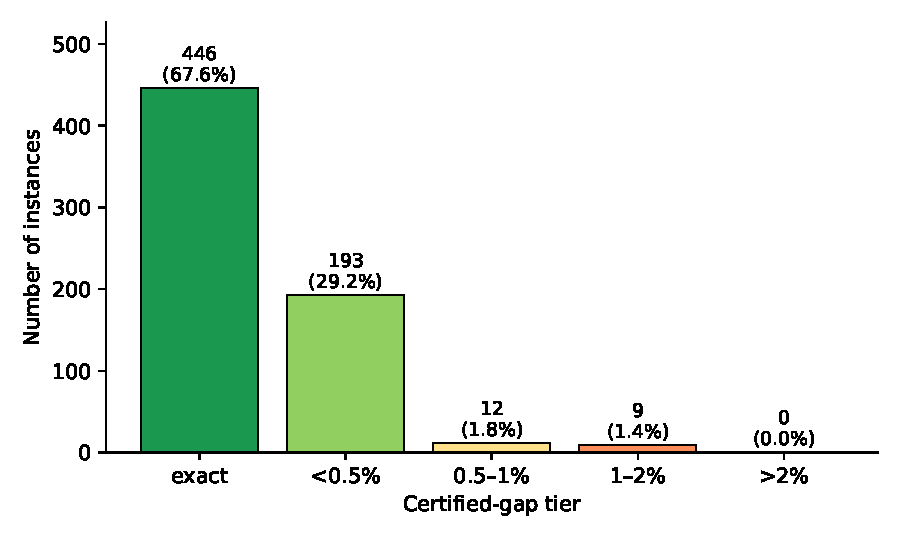
\includegraphics[width=0.72\linewidth]{figures/fig_cert_tiers.pdf}
\caption{Distribution of certified-gap tiers over the 660-instance study set. No instance falls above $2\%$; 67.6\% are certified exact and 96.8\% within $0.5\%$.}
\label{fig:certtiers}
\end{figure}

\subsection{Gap and comparison conventions}
\label{subsec:gap-defs}

We distinguish three related quantities. First, the exact BPC algorithm reports a
primal--dual gap of $100\times(\text{dual}-\text{primal})/\text{primal}$ on each
instance \cite{RieraLedesma2021SRPS}. Second, our certified gap is always computed as
\[
\text{cert\_gap} = \frac{UB_{\text{lag}} - z^*}{UB_{\text{lag}}} \times 100,
\]
where $UB_{\text{lag}}$ is the Lagrangian upper bound of
Section~\ref{sec:lagrangian} and $z^*$ is the objective value of the incumbent
feasible solution. This gap is a rigorous bound on suboptimality because
$UB_{\text{lag}}$ is never taken below any known feasible objective.

Third, when comparing against published best-known solutions (BKS) we report
$\Delta\text{obj} = z^* - \text{BKS}$, so positive values indicate an improvement
and negative values a shortfall. These conventions are used consistently in
Table~\ref{tab:mainresults} and Table~\ref{tab:bpcsplit}.

A per-instance table reporting objectives, bounds, gaps, stop reasons, and runtime splits is provided in the Supplementary Material. Certificates are deposited in the repository and are independently checked by evaluating $L(\mu)$ on the raw instance, without search or subgradient iteration.

\subsection{Certified optima and subproblem cost}

Of the 660 study instances, 446 (67.6\%) are returned with a certified gap of
exactly zero and are therefore proven optimal in the sense of
Section~\ref{sec:lagrangian}. Of those, 220 are also proved optimal by the exact
BPC method, where the two certificates coincide and cross-validate one another;
the remaining 226 are proven optimal by the Lagrangian certificate, without a corresponding BPC optimality proof published in the baseline study.

Agreement with BPC-proved optima is a useful falsification check, but it alone
does not establish the validity of a bound from a different method. The
repository deposits each multiplier vector and its incumbent. The Path-B check
independently reproduces all reported bounds from the raw instances and stored
multipliers. As falsification checks, no bound falls below its incumbent (660
instances), an external BKS (461), or a BPC-proved optimum (245), and
refinement never loosens the bound it replaces. These checks do not establish
the guarantee; that rests on Proposition~\ref{prop:main_valid} and exact
solution of the per-processor subproblems.

These certificates are not all produced the same way, and the distinction is
worth stating because it separates what the construction achieves from what the
adaptive loop achieves. On 155 of the 660 instances the greedy construction
already meets the initial decomposition bound, so the instance is certified
optimal by the pre-search guard of Algorithm~\ref{alg:solver}, without an ALNS
phase or a subgradient step ever being executed; these solve in a median of $0.7$ seconds.
They account for 155 of the 446 proven-optimal results, and they pull the
headline median runtime down: the median over all 660 instances is $6.2$ minutes,
while the median over the 505 instances that do enter the loop is $10.2$ minutes.
The adaptive loop and the refinement stage should therefore be read against those
505 instances, on which the remaining 291 optimality proofs and every nonzero
certificate are obtained. That a quarter of the benchmark is certified in under a
second is itself a useful property of the decomposition bound, but it is a
property of the bound and the construction, not of the search.

The validity of each evaluated Lagrangian bound requires exact solution of the per-processor subproblems; tightness depends on how far the truncated subgradient has converged. Both properties are served by keeping the per-processor job sets small,
and they do. Across all 660 instances the largest $|J_k|$ is $13$, with
per-instance means of $2.8$--$6.0$, and this maximum is \emph{flat in $n$}: it is
already $13$ at $n=80$ and remains $13$ at $n=150$. Each subproblem therefore
costs at most $2^{13}\cdot 13^2\approx 1.4\times10^{6}$ operations, so
$UB_{\text{lag}}$ is computed exactly---with no pruning, sampling, or
candidate-set restriction---even on the largest instances.

\subsection{Validation where optima are known, extension where they are not}

The exact method establishes ground truth on part of this benchmark and leaves the rest open, and Table~\ref{tab:bpcsplit} is best read in those two parts. Where BPC has proved an optimum, our result is a \emph{check on the method}. Where it has not, our result is the contribution.

\emph{Where the optimum is known.} Group~A contains the 245 instances BPC proves optimal. The present method matches the BPC-proved objective on 241 of them (A1); under the fixed one-hour budget, it terminates one profit unit below that value on four (A2), with a mean certified gap of 0.018\%. Thus it matches $98.4\%$ of independently proved optima, providing a stringent validation of the primal search while transparently retaining four bounded-budget misses. The dual certificates' validity is established independently by Proposition~\ref{prop:main_valid}, which does not depend on any comparison against known optima. A certified heuristic on an instance already closed by an exact method provides an independent dual certificate but not a new primal result.

\emph{Where it is not.} The remaining $415$ instances ($412$ in groups B and C plus three partially-solved instances noted in the Table~\ref{tab:bpcsplit} footnote) are where the method earns its place. Group~B contains 112 instances where BPC returns an incumbent but stops at the one-hour limit with a nonzero gap; here the present method matches the reported incumbent on 93 (B2), improves it on 15 (B1), and is one profit unit below on four (B3), certifying every one of them to a mean gap of 0.129\% --- so instances that were left with an open primal--dual gap now carry a bound. Group~C contains 300 instances with no reported BPC solution\footnote{That is, no result is published for these instances under the exact method's original one-hour campaign; this does not assert that no feasible solution exists or that the exact method could not find one under a different setup.}; the present method certifies all 300, including 196 first-ever certified results. On the 104 Group~C instances with an external published BKS, the method improves nine, matches 91, and is below four.

BPC's published primal--dual gaps and the present certified gaps are not numerically identical quantities, because they use different relaxations and denominators. We therefore report them side by side as context, while treating objective values and certified coverage as the primary comparative outputs.

\begin{table}[t]
\centering
\setlength{\tabcolsep}{5pt}\small
\caption{Coverage relative to the exact BPC baseline (660 study instances), grouped by what the exact method establishes: proved optima (A, where our result validates the method), an incumbent with an open gap (B), and no reported result (C). $\Delta$obj is our objective minus the best known solution (BKS); certified gaps are reported against a validity-guarded upper bound (never taken below a known feasible objective). BPC times are its actual reported per-group CPU times (BPC-SRPS-E, under a 1\,h cap), averaged over each subgroup; our times are wall-clock on different hardware (Python, 6-core laptop, 2026) and are not comparable to BPC times (compiled C++/CPLEX on a single earlier-generation core). The meaningful cross-method comparisons are coverage, incumbent quality, and certified gaps, not runtimes. Our certified gaps and runtimes are the post-refinement values of Table~\ref{tab:mainresults}, on the same accounting as Section~\ref{sec:experiments}: the group means weight to the 0.066\% headline.}
\label{tab:bpcsplit}
\fittable{%
\begin{tabular}{llrrrr}
\toprule
\multicolumn{2}{l}{Outcome group / subgroup} & $n$ & $\Delta$obj vs BKS & Cert.\ gap & Our / BPC time \\
\midrule
\multicolumn{2}{l}{\textbf{A.\ BPC proves optimal}} & 245 & $0$ & 0.018\% & 316 / 32\,s \\
& A1\quad recover optimum ($=$BKS) & 241 & $0$ & 0.017\% & 315 / 32\,s \\
& A2\quad miss optimum ($<$BKS) & 4 & $-1$\,($-0.04\%$) & 0.056\% & 401 / 34\,s \\
\midrule
\multicolumn{2}{l}{\textbf{B.\ BPC incumbent, gap at 1\,h cap}} & 112 & $+3.6$ & 0.129\% & 572 / 1415\,s \\
& B1\quad improves BKS & 15 & $+27$\,($+0.95\%$) & 0.193\% & 718 / 1930\,s \\
& B2\quad matches BKS & 93 & $0$ & 0.118\% & 541 / 1324\,s \\
& B3\quad below BKS & 4 & $-1$\,($-0.03\%$) & 0.158\% & 745 / 1609\,s \\
\midrule
\multicolumn{2}{l}{\textbf{C.\ BPC provides no reported incumbent}$^{\dagger}$} & 300 & --- & 0.081\% & 656 / ---\,s \\
& \multicolumn{5}{l}{\footnotesize 196 first-ever certified; of the 104 with a BKS: 9 improve, 91 match, 4 below} \\
\bottomrule
\end{tabular}%
}

\smallskip
{\footnotesize $^{\dagger}$Three further instances belong to BPC groups that were only partially solved, so no per-instance BPC result is attributable to them; the present method certifies all three (mean 0.166\%). They lie within the 415 open/unreported instances and are grouped with~C, but are excluded from its count and from the 196 first-ever tally.}
\end{table}

\subsection{Independent verification against a general-purpose MIP solver}

The comparisons above rest on values published for the exact method. As an
external check that does not depend on those figures, we solved the compact
arc-flow model SRPS-1 directly with CPLEX~22.1.1 and compared both its
incumbents and its dual bound against ours. The check is deliberately
uncoupled: the model is built from the instance file alone and shares no code,
data structure, or intermediate state with either the ALNS or the Lagrangian
scheme.

We ran it on the 30 study instances with $n\le 50$ that still carry a nonzero
certified gap, under a 180-second limit on six threads. This is an external
sanity check, not a controlled comparison with the single-threaded one-hour BPC
campaign. Instances already
certified optimal are excluded, since for those there is nothing to verify.

Within that limit CPLEX closed 7 of the 30. On those seven the present method's
incumbent is \emph{provably optimal} on five; on one it is one profit unit below
the optimum, and on one (\texttt{ED\_n040\_004\_a50\_011}) ten units below.
Across the 23 instances CPLEX could not close, it matched our incumbent on 12,
fell below it on 10, and exceeded it on one. Taken together, on 27 of the 30
instances the two methods agree or the present method is ahead, and on three it
is behind. This is consistent with the BKS-based comparison of
Table~\ref{tab:bpcsplit} while resting on an entirely independent solver.

The bound comparison is the more informative half. On 22 of the 30 instances the
Lagrangian certificate is \emph{strictly tighter} than the dual bound CPLEX
attains within its limit. That ordering is not accidental. The Lagrangian
subproblem is an orienteering problem over a single processor, solved to
optimality by bitmask dynamic programming, and the orienteering polytope does
not have the integrality property \cite{Geoffrion1974Lagrangean};
consequently the Lagrangian bound may
strictly dominate the linear relaxation of the compact model, and here it
generally does. The same structural weakness of SRPS-1 is why the exact
literature attacks the problem by branch-price-and-cut
\cite{Barnhart1998BranchPrice} rather than by solving the compact formulation
directly \cite{RieraLedesma2021SRPS}.

Two limits should be stated. The check covers small instances only: a compact
MILP is not competitive at the sizes where our certificates matter most, and the
specialised exact method itself closes only $n\le 60$. And a 180-second limit is
short by exact-solver standards, so the bound comparison should be read as
``tighter than a general-purpose solver derives from SRPS-1 in the time our
method takes overall'', not as a claim about CPLEX's asymptotic behaviour.

\subsection{New certified results on open instances}

For line instances D with $n=65$--80 and Euclidean instances ED with $n=65$--80, the method supplies certified solutions throughout the open range, 114 of which have no previously published best-known value. Several are certified with very small gaps; for example, the line instance D\_n075\_037 at $\alpha=0.75$ is certified within 0.04\% of optimal, and multiple $n=65$ instances are certified exact. Representative entries are listed in Table~\ref{tab:newresults}.

The method also improves 24 published incumbents. Table~\ref{tab:newresults} reports representative entries and their certified gaps.

\begin{table}[t]
\centering
\caption{Representative first-ever and improved certified solutions. ``new'' = no previously published best-known value; ``improved'' = improves a published incumbent (margin over the old value in the note).}
\label{tab:newresults}
\fittable{%
\begin{tabular}{lccccl}
\toprule
Instance & Objective & $UB_{\text{lag}}$ & Cert. gap & Status & Note \\
\midrule
D\_n065\_026\_a50  & 1848 & 1848 & 0.00\% & new  & first-ever, proven optimal \\
D\_n075\_037\_a75  & 2337 & 2338 & 0.04\% & new  & near-optimal large line instance \\
ED\_n065\_026\_a75 & 1900 & 1901 & 0.05\% & improved &$+11.8\%$ over published BKS (1699) \\
EB\_n140\_024\_a50 & 5525 & 5535 & 0.18\% & improved &$+9.8\%$ over published BKS (5034) \\
EB\_n140\_022\_a50 & 4900 & 4922 & 0.45\% & improved &$+8.8\%$ over published BKS (4503) \\
\bottomrule
\end{tabular}%
}
\end{table}

\subsection{Effect of in-loop re-bounding}

The Lagrangian bound is what makes the method a certified primal--dual solver rather than a high-quality heuristic; the in-loop re-bound then sharpens that certificate specifically on the hard tail of the benchmark, namely instances that remain difficult after a full ALNS phase and therefore trigger multiplier refreshes and destroy-tier escalation (the 70 instances that stop at tier exhaustion). The empirical outcome is that every one of the 660 study instances is certified within 2\%, even though the hardest cases occur at tight budgets and larger sizes.

To isolate the contribution of the in-loop re-bound, we re-ran \emph{every} one of the 70 hard-tail instances with it disabled --- a census of that stratum rather than a sample --- the upper bound is computed once and never re-tightened --- holding everything else fixed and warm-starting both arms identically. Table~\ref{tab:hardtail-refresh} reports the outcome. Disabling the in-loop re-bound raises the mean certified gap on the hard tail from 0.691\% to 0.955\%, a mean reduction of 0.264 percentage points attributable to the re-bound (median 0.196, maximum 1.457). The re-bound tightens the certificate on 53 of the 70 instances and is what brings 22 of them below a 1\% certified gap and 16 below 0.5\%, while leaving 11 unchanged. On the remaining six the certified gap is marginally larger with the re-bound enabled (by at most 0.18 pp); this reflects run-to-run variation in the stochastic primal search rather than the bound itself, since the re-bound can only tighten the dual value. The effect is thus consistent and, on the hardest instances, substantial. It is also purely dual: the returned objective is identical in both arms on all $70$ instances, so the re-bound buys certificate rather than solution --- which is what a bound-tightening mechanism should do, and is the reason it is invisible to any ablation scored against a common bound. It is by construction a certificate-tightening mechanism, which is why it has a near-zero effect in the fixed-bound ablation of Section~\ref{sec:experiments}, where the upper bound is held common across arms.

Two clarifications belong with this experiment. First, it is conducted on the certificates \emph{before} the refinement stage, for the same reason as the hardness analysis: it isolates the contribution of the in-loop mechanism, and refinement is applied uniformly afterwards to both arms. The gaps quoted here are therefore larger than the headline figures of Table~\ref{tab:mainresults}, which are post-refinement. Second, the two mechanisms are not substitutes: the refreshed bound is what the stopping rule reads, so removing it changes \emph{when the search stops}, not merely how tight the final certificate is, whereas refinement runs only after termination and cannot influence the search at all.

\begin{table}[t]
\centering
\caption{Effect of the in-loop Lagrangian re-bound on the 70 hard-tail instances (TIERS\_EXHAUSTED). Both arms start from the same initial upper bound; the no-refresh arm never re-tightens it. $\Delta\text{gap}=\text{gap}_{\text{no-refresh}}-\text{gap}_{\text{full}}$.}
\label{tab:hardtail-refresh}
\begin{tabular}{lr}
\hline
Quantity & Value \\
\hline
Instances & 70 \\
Mean certified gap, full & 0.691\% \\
Mean certified gap, no-refresh & 0.955\% \\
Mean gap reduction $\Delta$ & 0.264 pp \\
Median gap reduction $\Delta$ & 0.196 pp \\
Max gap reduction $\Delta$ & 1.457 pp \\
Instances improved / unchanged / worsened & 53 / 11 / 6 \\
Crossings to $<$1\% / $<$0.5\% / exact & 22 / 16 / 0 \\
\hline
\end{tabular}
\end{table}

\subsection{Ablation, sensitivity, and hardness summary}

\paragraph{Ejection chain} One component is evaluated in closed form rather than by running an arm. The ejection chain is a post-loop pass whose gain is recorded per instance; because the objective is a sum of integral profits and the certified gap is linear in it, removing the component changes the gap by exactly $\text{ec\_gain}/UB$ --- an identity, evaluable on all $660$ instances rather than only the ablation subset. The final pass improved the returned incumbent on $12$ of the $660$ instances: $0.0000$ percentage points of certified gap on the $70$ hard-tail instances (it never fires there) and $0.0008$ points on the full study set. The consequence that matters is discrete: three of the $446$ proven-optimal results depend on it, each closed by the single profit unit it supplies.

\paragraph{Ablation study} Arms are evaluated on a stratified $40$-instance sample (fixed seed): $20$ of the $70$ hard-tail instances and $20$ of the $198$ multi-phase instances that still close, reported separately and never pooled, against a common fixed certified bound. The measured hard-tail noise floor (disjoint-seed replicate, Supplementary Material) is a mean $|\Delta|=0.036$\,pp, implying a minimum detectable effect at this sample size of $0.084$\,pp. Table~\ref{tab:ablation} reports the mean marginal effect of removing each component. Repair-pool diversity (B4) dominates by roughly two orders of magnitude, costing $2.49$--$2.50$\,pp in both strata and changing the search's own stop reason on $45\%$ of the sample; the all-off arm (S) is $2.51$--$2.53$\,pp, essentially equal to B4 alone, and the marginal components sum to within $4$--$5\%$ of that total (additive, not a hidden interaction). Every other component falls at or below the detection floor except B2 (greedy acceptance, i.e.\ SA disabled), at $+0.10$\,pp on the hard tail.

\begin{table}[h]
\centering
\caption{Mean marginal effect of removing each component ($\Delta$gap vs.\ A0,
pp, common certified bound), $n=20$ per stratum. Minimum detectable effect at
this sample size: $0.084$\,pp.}
\label{tab:ablation}
\fittable{%
\begin{tabular}{lrrrrrrrrr}
\toprule
Stratum & B1 & B2 & B3 & B4 & B5 & B6 & B7 & B8 & S \\
\midrule
Hard tail & $+0.02$ & $+0.10$ & $-0.01$ & $+2.49$ & $+0.00$ & $+0.02$ & $0.00$ & $0.00$ & $+2.51$ \\
Closing   & $-0.01$ & $+0.01$ & $+0.01$ & $+2.50$ & $+0.01$ & $+0.02$ & $+0.00$ & $0.00$ & $+2.53$ \\
\bottomrule
\end{tabular}%
}
\end{table}

A pooled null does not mean a component never acts: counted per instance against the same floor rather than averaged, B1, B3 and B6 each exceed it on a nontrivial minority of instances (5--11 of 40) whose opposite-signed effects cancel in the mean; B5, B7 and B8 remain null by that finer count too, and B7 additionally changes the search's stop reason on zero of the $40$ instances --- the strongest evidence here that a component is inert rather than merely small on average. B5 and B7 also have a stronger, larger-population measurement already in hand (the ejection-chain identity above and the in-loop re-bound census of Table~\ref{tab:hardtail-refresh}); both were run as sampled arms here purely as a cross-check, and both agree with the stronger measurement. The full per-family/per-size breakdown, the cross-check detail, and the exploratory family-concentration pattern we found for B1/B2 are in the Supplementary Material.

\paragraph{Sensitivity study} A one-at-a-time sweep on a 30-instance stratified subset varies eleven parameters around the chosen defaults (Supplementary Material). Its resolution is measurable rather than assumed: a duplicated configuration measures a run-to-run noise floor of $0.005$\,pp, and nine of the eleven variants move the mean by less than that. The other two act by letting the search run longer rather than by changing how it searches (tightening the stopping threshold, worth $0.024$\,pp; lengthening the phase budget, worth about half that) and neither was adopted in production, since both push compute toward the per-instance runtime cap. These gap figures are measured before the post-search refinement stage and the in-loop monotonicity guard existed; since refinement only re-solves the dual against a fixed incumbent and the primal search code is otherwise unchanged, we cross-checked the same trials on primal objective value alone (Supplementary Material): ten of the eleven variants reproduce the production reference incumbent within $0.01\%$, and only the longer phase budget shows a clear effect, consistent with the gap-based finding. The hard-tail noise floor is measured independently at a mean $|\Delta|=0.036$\,pp (Supplementary Material) and is larger than the $0.005$\,pp figure here, which is consistent: the 30-instance subset is dominated by instances whose certificate does not depend on these parameters, so its measured variance underestimates the true run-to-run noise where parameters can act.

\paragraph{Hardness} Certification difficulty is driven overwhelmingly by budget tightness. Figure~\ref{fig:hardness} shows the pattern directly: at $\alpha=0.75$ certified gaps collapse to near zero across every family, while the hardest cells sit at $\alpha=0.25$, and residual variation is shaped by an interaction between budget tightness and distance geometry. A censored regression on the pre-refinement certificates supports the same ordering, but we report it no further than this: the effect is estimated on the series \emph{before} refinement, and on the refined certificates the paper actually reports---censored at zero on $446$ of $660$ observations---the budget term is no longer separately identified. The descriptive pattern is robust; the model behind it is diagnostic, and we do not rest any claim on it.

\begin{figure}[t]
\centering
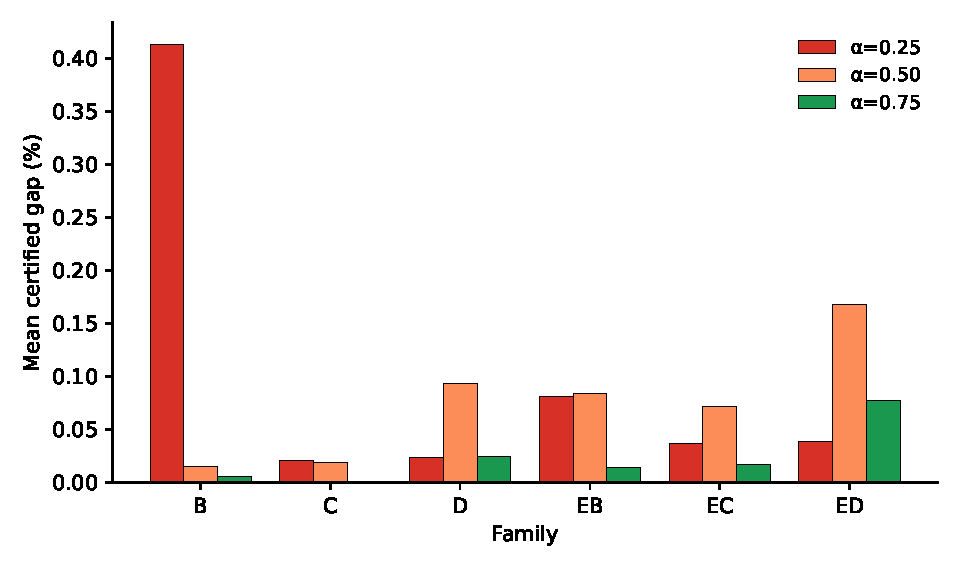
\includegraphics[width=0.78\linewidth]{figures/fig_hardness.pdf}
\caption{Mean certified gap by family and budget tightness $\alpha$. Budget tightness dominates ($\alpha=0.75$ collapses gaps across all families), and the Euclidean families (EB/EC/ED) retain more residual difficulty at a given $\alpha$ than their line counterparts, consistent with the $\alpha\times$distance interaction.}
\label{fig:hardness}
\end{figure}

\section{Discussion}\label{sec:discussion}

The computational evidence supports a complementary role relative to exact BPC, not a replacement claim. On instances where BPC proves optimality quickly, the present method mainly re-validates known optima; where BPC reaches its time limit with residual gaps or no reported solution, it contributes certified near-optimal incumbents. A practical workflow is therefore sequential: run the exact method first, then apply the certified heuristic on unresolved instances.

The objective comparisons and the bound comparisons should be interpreted separately. BPC's published primal--dual gaps and the present certified gaps are derived from different relaxations and different denominators, so they are not numerically identical metrics. The meaningful cross-method comparison is coverage and incumbent quality under certification, not a one-to-one gap-value equivalence.

Since the Lagrangian certificate is already exact on 67.6\% of instances and averages 0.066\%, any cut-based strengthening of the dual is bounded in advance by that margin. The bound is in fact sharper than the mean suggests. Because the optimum $P^*$ is known only to lie in $[z^*, UB_{\text{lag}}]$, the largest improvement available to \emph{any} technique acting on either end of that interval --- dual-side or primal-side --- is the certified gap itself, whose median over the study set is now zero: on the median instance the certificate is closed and there is provably nothing to recover. The total absolute headroom is $1125$ profit units across all $660$ instances, and $71\%$ of it is concentrated in fifty instances, so what remains is not only small but narrowly localised.

A second obstacle is structural rather than quantitative, and applies specifically to separation inside a primal heuristic. Cutting planes are separated against a current solution, and the solution this method maintains is feasible by construction: it violates no valid inequality, so a separation routine run against it returns an empty candidate set whatever the cut family. Useful separation would have to be directed at an infeasible object --- in this architecture the Lagrangian relaxed solution, whose per-processor routes are individually within the horizon but need not admit a common synchronised schedule. We therefore do not pursue BPC-style separation here, and record the directions that remain open in Section~\ref{sec:conclusion}.

The improved incumbents reported here should be read as benchmark updates, not as claims that the exact method is dominated. An improved published incumbent indicates that the recorded best-known value can be tightened, while the accompanying certificate quantifies proximity to optimality. This is especially relevant on the open class-4 frontier, where benchmark coverage rather than formal dominance is the main scientific value.

\section{Conclusions}\label{sec:conclusion}

To the best of our knowledge, this paper presents the first ALNS-based Lagrangian-certified heuristic for SRPS, combining a synchronisation-aware ALNS with a Lagrangian relaxation that provides valid, independently checkable per-instance upper bounds. The method is best understood as a complement to exact BPC: it reproduces exact results closely where they are known, and extends the benchmark with certified near-optimal solutions where the exact method leaves gaps or no published result. In practice the two are naturally used in sequence --- the exact solver wherever it terminates, and the present method on the larger, tighter-budget instances it leaves open.

The computational evidence is particularly strong on the hard and previously open instances, where the method delivers uniformly tight certificates at practical runtimes. More broadly, the results show that a heuristic search procedure can be coupled tightly enough to a dual bounding mechanism to yield a scalable solver with meaningful guarantees.

Several limitations remain. The method is not exact and offers no approximation ratio. The implementation is in Python, so absolute runtime comparisons reflect engineering choices as well as algorithmic ones. The present study is also benchmark-centric, relying on a single established SRPS testbed.

A further limitation concerns the dual budget, and we state it precisely because the obvious remedy does not work. Every certificate reported here is produced under an in-loop refresh capped at 200 subgradient iterations or 60 seconds, and probing the subgradient to 1000 iterations on the loosest-gap instances shows it still descending when that cap is reached. Measured in isolation the dual is therefore not converged, and a larger budget does tighten it. That gain does not transfer to the solver at a fixed per-instance runtime cap. Raising the wall-clock allowance of the refresh takes time directly from the primal search, and on instances that stall repeatedly the exchange is unfavourable: in a re-run at five times the dual time allowance, incumbents on the most dual-intensive instances were worse by several profit units on average and more instances lost proven-optimal status than gained it. Holding the wall-clock allowance fixed and raising only the iteration cap changes little, because on the large instances the subgradient completes fewer than 200 iterations within 60 seconds in any case, so the iteration cap is not the binding constraint where the headroom is. The certificate is tightenable in isolation, but not for free \emph{inside the loop} (Section~\ref{sec:certification}). The limitation is therefore real but bounded --- it constrains what the in-loop refresh can achieve, not what the method can certify.

Future work includes stronger exact--heuristic hybridisation, richer preprocessing, transferring the certification framework to related synchronised prize-collecting routing problems, and testing whether the same primal--dual architecture remains effective on broader real-world scheduling settings.

Two directions follow directly from the analysis above, and both target the same measured deficiency: the per-processor subproblem enforces route length exactly but is blind to synchronised idle time, which is where the residual looseness lives. Neither is a matter of spending more effort on the existing relaxation --- the refinement stage already does that, and what it leaves behind is structural rather than budgetary.

The first is Lagrangian \emph{decomposition}, but only under the right split: duplicating variables across the natural split cannot help, because the dualised joint-service block has the integrality property and the decomposition bound therefore coincides with the relaxation bound already computed \cite{GuignardKim1987LD,Geoffrion1974Lagrangean}, whereas separating routing from synchronisation timing dualises a copy constraint whose blocks both have non-integral hulls and admits strict improvement. The second is Benders decomposition \cite{Benders1962Partitioning}: fixing the selection and the per-processor routes leaves synchronisation feasibility as a difference-constraint system, a linear programme whose dual rays yield feasibility cuts directly. Both address the blindness itself rather than the resources given to a relaxation that cannot see the constraint in question.

\section*{CRediT authorship contribution statement}
\textbf{David Chouchena}: Software, Formal analysis, Investigation, Data curation, Writing~-- original draft.
\textbf{Yuval Ben-Abu}: Conceptualization, Methodology, Supervision, Validation, Writing~-- review \& editing.

\section*{Declaration of competing interest}
The authors declare that they have no known competing financial interests or personal relationships that could have appeared to influence the work reported in this paper.

\section*{Declaration of generative AI and AI-assisted technologies in the manuscript preparation process}
During the preparation of this work, the author(s) used GitHub Copilot (agentic mode, Claude-based) to assist with repository analysis, drafting and calibrating manuscript prose, writing analysis/reproduction scripts, and cross-checking numerical claims against source data. After using this tool, the author(s) reviewed and edited all content and take full responsibility for the content of the published article.

\section*{Data and code availability}
The benchmark instances are publicly available from Riera-Ledesma and Salazar-Gonz\'alez \cite{RieraLedesma2021SRPS} (\url{https://github.com/RieraULL/OPS-Benchmark}). The standalone solver, primary experiment drivers, certificate verifier, versioned certificates, and result-generating scripts are publicly available at
\url{https://github.com/chouchena/lagrangian-certified-alns-srps}. The repository's reproduction guide distinguishes deterministic recomputation of every current manuscript output from optional archived companion-workspace and CPLEX experiments.

\section*{Funding}
This work was supported by the Sapir Applied Science Institute, Faculty of Technology, Sapir Academic College, Israel. The funder had no role in the study design; the collection, analysis, or interpretation of data; the writing of this report; or the decision to submit the article for publication.

The article states the full SRPS model, the relaxed per-processor decomposition, and the central bound-validity proposition and proof in Section~3; the expanded algebraic derivation, the exact subproblem's bitmask dynamic-programming recurrence, and the floating-point safeguarding analysis behind the certified gap are given in the Supplementary Material.

\FloatBarrier

\bibliographystyle{elsarticle-num}
\bibliography{refs}

\end{document}
